\subsection{Generalizing Our Solution}

\begin{table}[t]
\centering
\caption{Comparison of the angle-cascade QCPINN model with the two classical models (Model-1 and  Model-2) for solving Wave, Klein-Gordon, and Convection-Diffusion Equations. The table presents the number of trainable parameters, relative $L_2$ error (\%), and final training loss for each model.}
\scriptsize
\begin{tabular}{@{}l
        c@{\hspace{12.0pt}}
        c@{\hspace{4.0pt}}@{\hspace{4.0pt}} |
        c@{\hspace{8.0pt}}
        c@{\hspace{8.0pt}}
        c@{\hspace{12.0pt}}
        c@{\hspace{8.0pt}}
        @{}}
        \toprule
\textbf{Problem} & \multicolumn{2}{c|}{\textbf{Method}} &\textbf{\makecell{\# Trainable \\Parameters}} & \multicolumn{2}{l}\textbf{\makecell{Relative $L_2$\\ Error(\%)}} & \textbf{\makecell{Final Training\\  Loss}}  \\
\midrule
        \multirow{4}{*}{\makecell{Wave \\Eq(\ref{eq:1DWave})}}  & \multicolumn{2}{c|}{\multirow{1}{*}{\textit{Cascade}}} & \multirow{1}{*}{771}  & u& $1.02e+01$ &  \multirow{1}{*}{$ 0.083$} \\
        \cline{2-7} \noalign{\vskip 1ex}
        &\multirow{2}{*}{{Classical}}& \multirow{1}{*}{Model-1}&\multirow{1}{*}{$7851$}  & u  & $2.06e+01$& \multirow{1}{*}{$ 0.128$} \\
        \cline{3-7} \noalign{\vskip 1ex}
        &&\multirow{1}{*}{ Model-2} &\multirow{1}{*}{2751}  & u  & $8.68e+00$& \multirow{1}{*}{$0.027$} \\
        \cline{1-7} \noalign{\vskip 1ex}
        \multirow{8}{*}{\makecell{Klein-Gordon\\ Eq(\ref{eq:Klein-Gordon})}}  & \multicolumn{2}{c|}{\multirow{2}{*}{\textit{Cascade}}} & \multirow{2}{*}{771}  & u& $1.17e+01$ &  \multirow{2}{*}{$2.727$} \\
        &  &  && f& $3.17e+00$ &  \multirow{2}{*}{} \\
        \cline{2-7} \noalign{\vskip 1ex}
        &\multirow{4}{*}{{Classical }}& \multirow{2}{*}{Model-1}&\multirow{2}{*}{7851}  & u  & $1.75e+01$& \multirow{2}{*}{$0.718$} \\
        &  &  && f& $3.35e+00$ &  \\
        \cline{3-7} \noalign{\vskip 1ex}
        &&\multirow{2}{*}{{Model-2}}& \multirow{2}{*}{2751}  & u  & $1.76e+01$& \multirow{2}{*}{$0.358$} \\
        &  &  && f& $3.78e+00$ &  \\
        \cline{1-7} \noalign{\vskip 1ex}
        \multirow{6}{*}{\makecell{Convection Diffusion \\Eq(\ref{eq:Convection-Diffusion})}}  & \multicolumn{2}{c|}{\multirow{2}{*}{\textit{Cascade}}} & \multirow{2}{*}{821}  & u& $1.20e+01$ &  \multirow{2}{*}{$0.008$} \\
        &  &  && f& $ 4.38e+00$ &  \multirow{2}{*}{} \\
        \cline{2-7} \noalign{\vskip 1ex}
        &\multirow{4}{*}{{Classical}}&  \multirow{2}{*}{Model-1}&\multirow{2}{*}{7901}  & u  & $ 2.00e+01$& \multirow{2}{*}{$0.014$} \\
        &  &  && f& $3.11e+00$ &  \\
        \cline{3-7} \noalign{\vskip 1ex}
        &&\multirow{2}{*}{{Model-2}}& \multirow{2}{*}{2801}  & u  & $2.06e+01$& \multirow{2}{*}{$0.1$} \\
        &  &  && f& $1.31e+01$ &  \\
        \bottomrule
\label{tab:more_cases}
\end{tabular}
\end{table}


 \begin{figure}[t]
    \centering
    \begin{tabular}{ccc}
        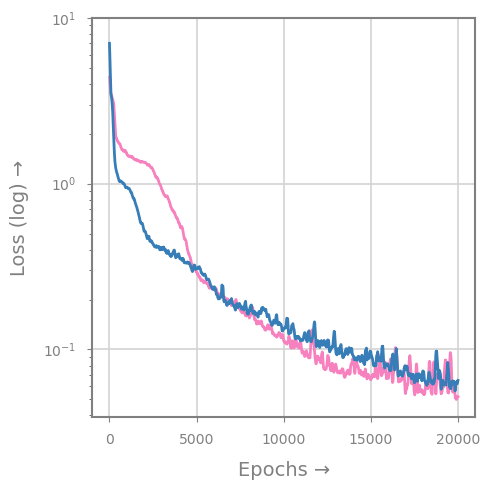
\includegraphics[width=0.3\columnwidth, trim={0cm .10cm 0cm 0cm}, clip]{figures/loss_history_wave.png} &
        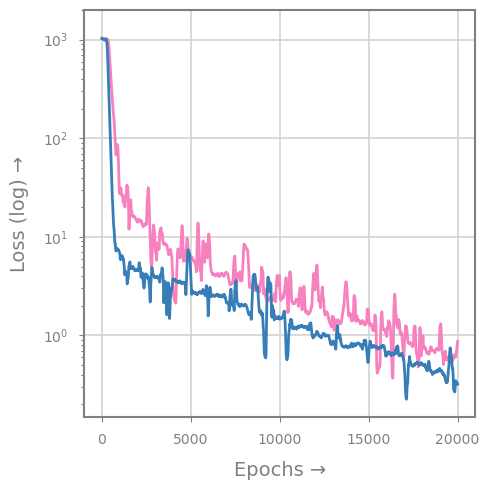
\includegraphics[width=0.3\columnwidth, trim={0cm .10cm 0cm 0cm}, clip]{figures/loss_history_klein.png} &
        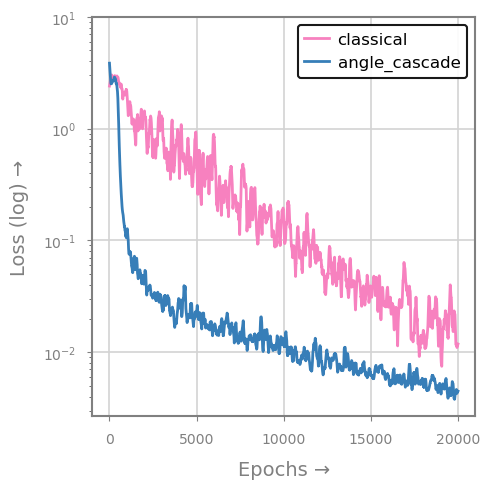
\includegraphics[width=0.3\columnwidth, trim={0cm .10cm 0cm 0cm}, clip]{figures/loss_history_diffusion.png} \\
        \footnotesize{(a) Wave} & \footnotesize{(b) Klein-Gordon} & \footnotesize{(c) Convection Diffusion}
    \end{tabular}
    \caption{ Training loss history for the (a) Wave equation, (b) Klein-Gordon equation, and (c) Convection-Diffusion equation. The plots compare the convergence behavior of the classical model's best testing results shown in table~\ref{tab:more_cases} and angle-cascade QCPINN models over 20,000 training epochs.}

    \label{fig:more_cases_loss_history}
 \end{figure}

 \begin{figure}[t]
    \centering
    \begin{tabular}{c}
        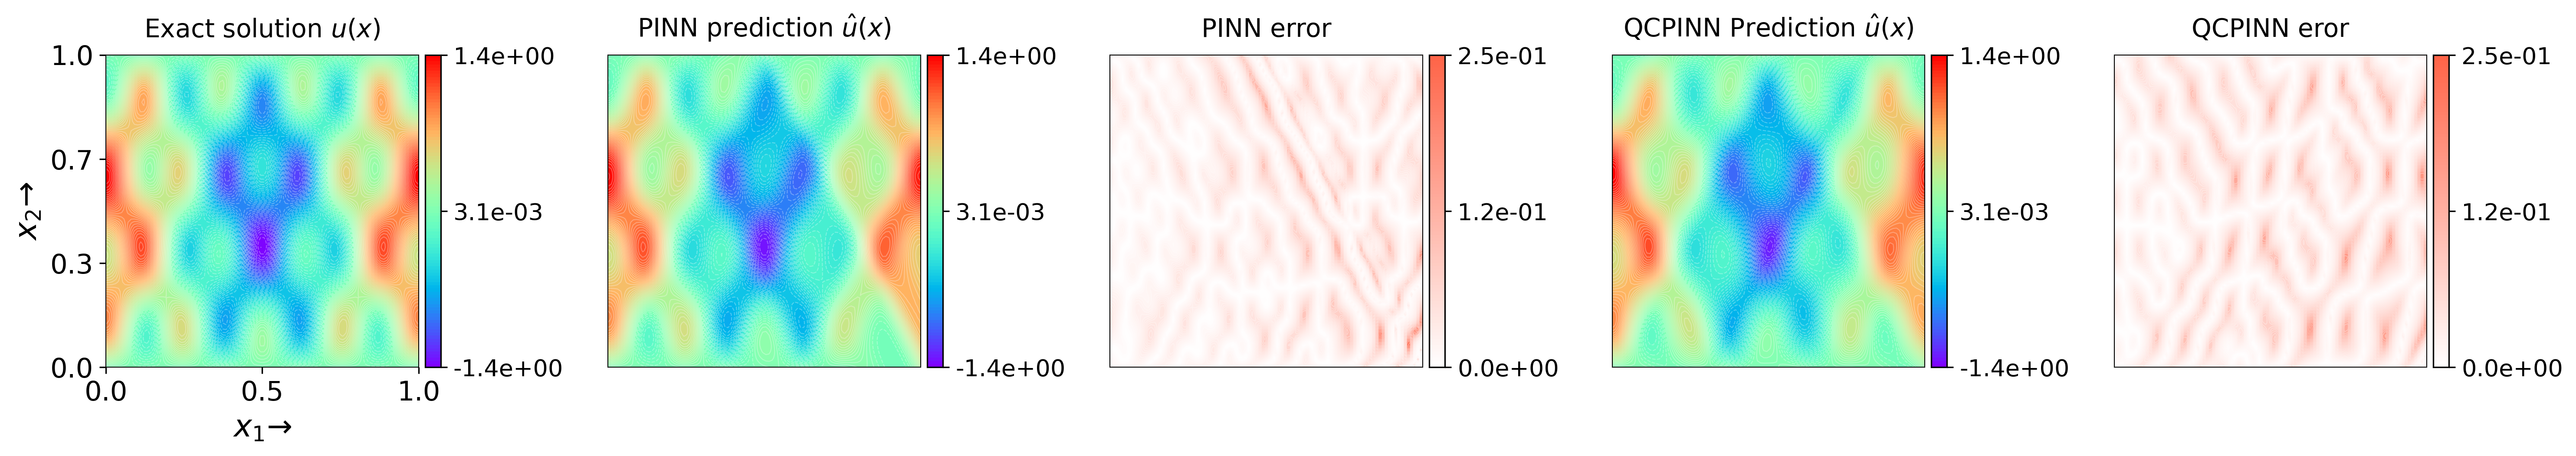
\includegraphics[width=0.81\columnwidth, trim={0.2cm 0.3cm 0.2cm 0.2cm}, clip]{figures/prediction_wave.png}  \\   
        \footnotesize{(a) Wave} \\ 

        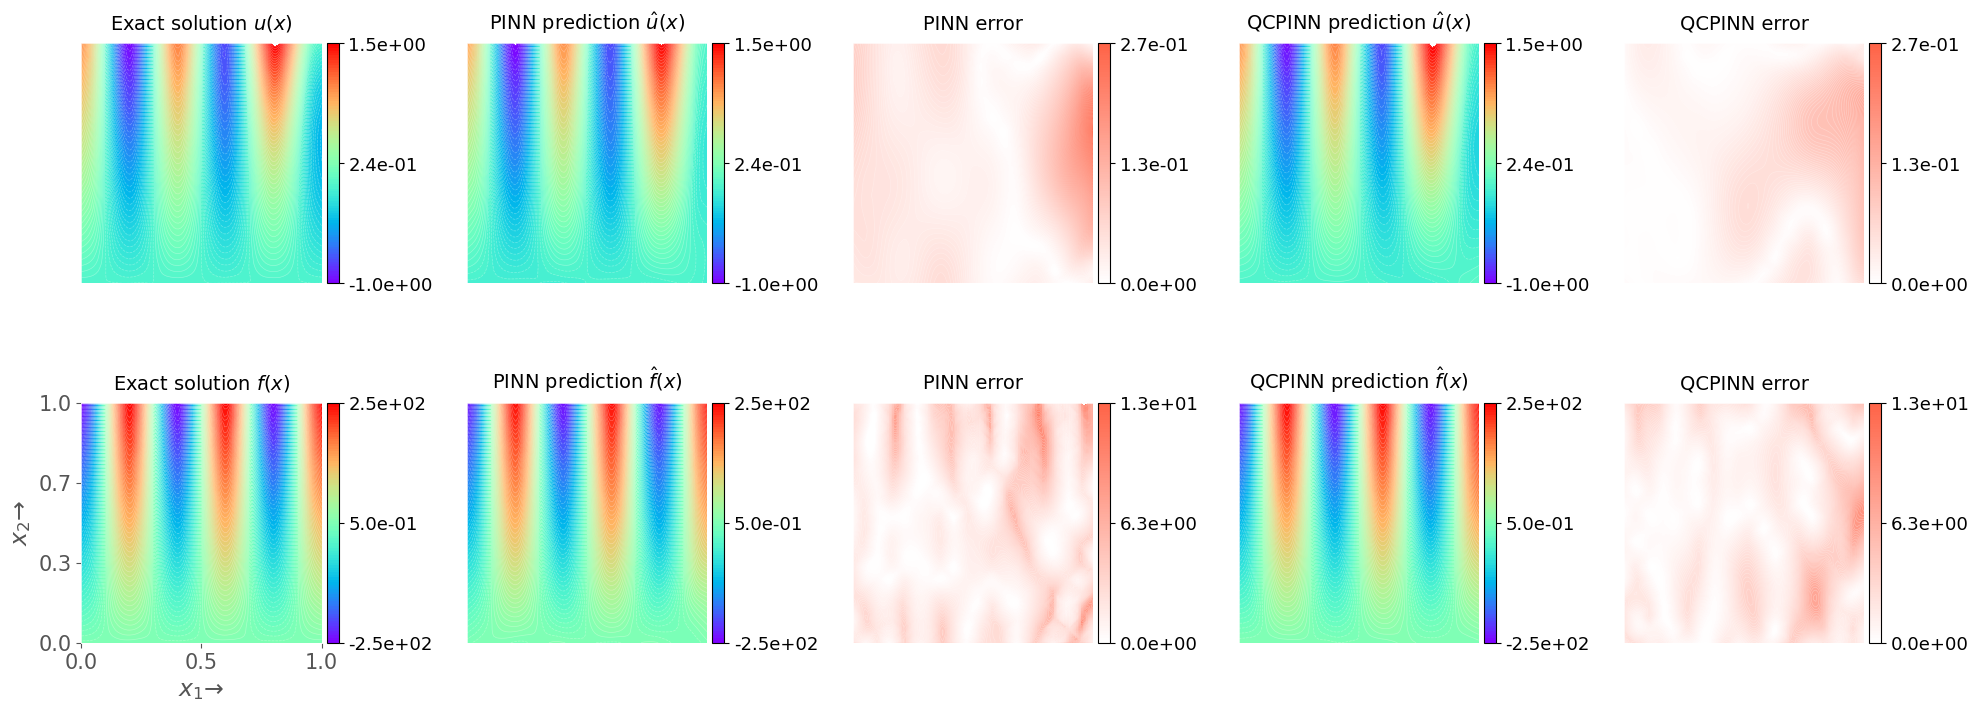
\includegraphics[width=0.81\columnwidth, trim={0.2cm 0.3cm 0.2cm 0.0cm}, clip]{figures/prediction_klein_gordon.png}   \\  
        \footnotesize{(b) Klein-Gordon} \\

        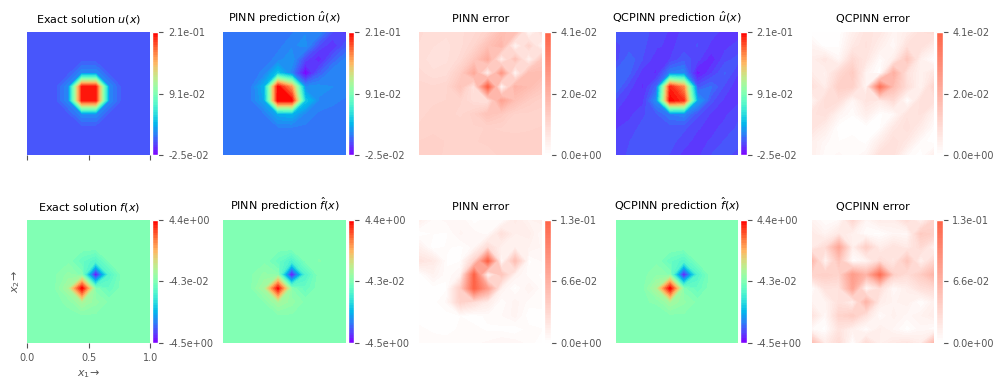
\includegraphics[width=0.81\columnwidth, trim={0.2cm 0.3cm 0.2cm 0.0cm}, clip]{figures/prediction_diffusion.png} \\
        \footnotesize{(c) Convection-Diffusion} \\
    
    \end{tabular}
    \caption{Comparison of the exact and predicted solutions using the best classical PINN results and angle-cascade QCPINN models. The first row corresponds to the solution \( u(x) \), while the second row represents \( f(x) \)(the exact force in wave equation is zero.)}

    \label{fig:more_cases_results}
 \end{figure}


Based on the results observed in our experiments with the Helmholtz and Cavity problems in~\ref{subsec:results_helmholtz} and \ref{subsec:results_cavity}, we identified that the angle-cascade QCPINN architecture consistently demonstrated better performance. To validate the robustness of our approach across diverse physical systems, we extended our evaluation to three additional canonical PDEs: the Wave equation~(\ref{eq:1DWave}), the Klein-Gordon equation~(\ref{eq:Klein-Gordon}), and the Convection-Diffusion equation~(\ref{eq:Convection-Diffusion}). This expansion allows us to assess whether the advantages of our quantum-enhanced architecture persist across problems with fundamentally different physical characteristics and computational challenges.

As evidenced in table~\ref{tab:more_cases}, our angle-cascade QCPINN model maintains its parameter efficiency advantage while achieving competitive orbetter accuracy compared to classical PINN approaches. For the Wave equation, our model requires merely 771 parameters, a 90.2\% reduction from the 7851 parameters of Classical Model-1, while achieving a relative $L_2$ error of 1.02e+1\% compared to 2.06e+1\% in the classical counterpart, representing a 50.5\% error reduction.
The Klein-Gordon equation presents additional complexity due to its coupled system nature. While our model shows marginally higher final training loss (2.727 versus 0.718), it maintains comparable relative $L_2$ errors for both solution components (u and f) while using only 9.8\% of the parameters required by Classical Model-1.
Most notably, for the Convection-Diffusion equation, our angle-cascade QCPINN with 821 parameters (versus 7901 in Classical Model-1) achieves a 40\% reduction in relative $L_2$ error for the primary solution variable (1.20e+01\% versus 2.00e+01\%) and demonstrates better training convergence with a final loss of 0.008 compared to 0.014 for Classical Model-1 and 0.1 for Model-2.

The Klein-Gordon equation presents additional complexity due to its coupled system nature. While our model shows marginally higher final training loss (2.727 versus 0.718), it maintains comparable relative $L_2$  errors for both solution components (u and f) while using only 9.8\% of the parameters required by Classical Model-1.
Most notably, for the Convection-Diffusion equation, our angle-cascade QCPINN with 821 parameters (versus 7901 in Classical Model-1) achieves a 40\% reduction in relative $L_2$  error for the primary solution variable (1.20e+01\% versus 2.00e+01\%) and demonstrates better training convergence with a final loss of 0.008 compared to 0.014 for Classical Model-1 and 0.1 for Model-2.

Figure~\ref{fig:more_cases_loss_history} provides insights into the convergence behavior of our models across all three equations. For the Wave equation (figure~\ref{fig:more_cases_loss_history}a), the angle-cascade QCPINN (blue line) exhibits significantly faster initial convergence, reaching lower loss values within the first 5,000 epochs compared to the classical approach (pink line). While both models eventually achieve similar final losses after 20,000 epochs, the quantum-enhanced model's accelerated early convergence represents a substantial computational advantage.
Similarly, the Klein-Gordon equation (figure~\ref{fig:more_cases_loss_history}b) demonstrates that our angle-cascade QCPINN maintains comparable convergence stability despite the equation's coupled nature, with both approaches showing similar loss trajectories after the initial training phase. Most impressively, for the Convection-Diffusion equation (figure~\ref{fig:more_cases_loss_history}c), our model maintains consistent and monotonic loss reduction throughout training, achieving a final loss approximately one order of magnitude lower than the classical approach.

Figure~\ref{fig:more_cases_results} visualizes exact and predicted solutions. For the Wave equation (figure~\ref{fig:more_cases_results}a), both models capture the oscillatory pattern, but the QCPINN error distribution (rightmost panel) shows noticeably lower error magnitudes across the domain. The Klein-Gordon equation results (figure~\ref{fig:more_cases_results}b) demonstrate our model's ability to accurately represent coupled solutions with error distributions comparable to or better than classical approaches.
The Convection-Diffusion equation results (figure~\ref{fig:more_cases_results}c) are particularly noteworthy, as they showcase our model's ability to capture the sharp localized features characteristic of convection-dominated flows precisely. The error visualization confirms significantly reduced prediction errors across both solution components (u and f), with error magnitudes approximately 2-3× lower than those of classical PINNs.

Beyond parameter efficiency, our angle-cascade QCPINN architecture substantially improves computational requirements. The reduction in trainable parameters directly translates to decreased memory consumption (up to 90\% reduction) and accelerated forward passes during training and inference. This efficiency advantage becomes increasingly significant for larger-scale physical systems where memory constraints often limit classical approaches.

These comprehensive results demonstrate that our angle-cascade QCPINN approach successfully generalizes across diverse PDE types, consistently delivering comparable or better solution accuracy while requiring significantly fewer parameters than classical alternatives. This parameter efficiency, combined with improved convergence properties for complex physical systems, establishes quantum-enhanced physics-informed neural networks as a promising direction for computational physics.
